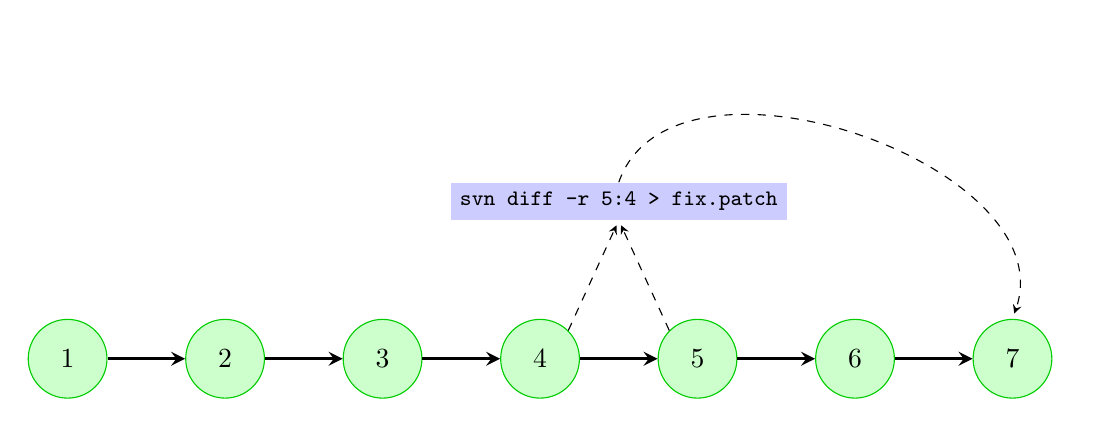
\begin{tikzpicture}
[rev/.style = {circle,
		draw=green!80!black,
		minimum size=10mm,
		fill=green!20!white},
 op/.style  = {fill=blue!20},
 trans/.style = {->,very thick,>=stealth}]
% line of development
\node[rev] at (0,0) (rev1) [] {1};
\node[rev] at (2,0) (rev2) [] {2};
\draw [trans] (rev1.east) -- (rev2.west);
\node[rev] at (4,0) (rev3) [] {3};
\draw [trans] (rev2.east) -- (rev3.west);
\node[rev] at (6,0) (rev4) [] {4};
\draw [trans] (rev3.east) -- (rev4.west);
\node[rev] at (8,0) (rev5) [] {5};
\draw [trans] (rev4.east) -- (rev5.west);
\node[rev] at (10,0) (rev6) [] {6};
\draw [trans] (rev5.east) -- (rev6.west);
% diff between revisions 4 and 5
\node[op] at (7, 2) (diff) {\footnotesize\texttt{svn diff -r 5:4 > fix.patch}};
\draw [->,>=stealth,dashed,shorten >=2pt] (rev4.north east) -- (diff.south);
\draw [->,>=stealth,dashed,shorten >=2pt] (rev5.north west) -- (diff.south);
% revision 7
\node[rev] at (12,0) (rev7) [] {7};
\draw [trans] (rev6.east) -- (rev7.west);
% fast forward to revision 7
\draw [->,>=stealth,dashed,shorten >=2pt,bend left=90] (diff.north) to (rev7.north);
\end{tikzpicture}
